% Practice Test 17 — Virginia Edition
% Questions: 30 (19 MC + 11 SA)
% Generated by scripts/generate_practice_tests.py

\begin{practiceQuestion}{1-4-q27}{gmc}
\begin{questionText}
The table below shows a proportional relationship. Using the equation, what is $y$ when $x = 9$?

\begin{center}
\begin{tabular}{|c|c|}
\hline $x$ & $y$ \\ \hline
$2$ & $11$ \\ \hline
$5$ & $27.5$ \\ \hline
$7$ & $38.5$ \\ \hline
\end{tabular}
\end{center}
\end{questionText}
\choiceA{$y = 45$}
\choiceB{$y = 49.5$}
\choiceC{$y = 54$}
\choiceD{$y = 63$}
\correctAnswer{B}
\explanation{$k = \frac{11}{2} = 5.5$. Equation: $y = 5.5x$. When $x = 9$: $y = 5.5 \times 9 = 49.5$.}
\end{practiceQuestion}

\begin{practiceQuestion}{2-1-q29}{gsa}
\begin{questionText}
Look at the $10 \times 10$ grid below. What percent of the grid is \textbf{not} shaded?

\begin{center}
\begin{tikzpicture}[scale=0.35]
  \foreach \x in {0,...,9} {
    \foreach \y in {0,...,9} {
      \draw[gray!50] (\x,\y) rectangle (\x+1,\y+1);
    }
  }
  % Shade 72 squares (rows 0-6 full = 70, plus 2 in row 7)
  \foreach \x in {0,...,9} {
    \foreach \y in {0,...,6} {
      \fill[funOrange!40] (\x,\y) rectangle (\x+1,\y+1);
      \draw[gray!50] (\x,\y) rectangle (\x+1,\y+1);
    }
  }
  \foreach \x in {0,...,1} {
    \fill[funOrange!40] (\x,7) rectangle (\x+1,8);
    \draw[gray!50] (\x,7) rectangle (\x+1,8);
  }
\end{tikzpicture}
\end{center}
\end{questionText}
\correctAnswer{$28\%$}
\explanation{Shaded squares: $7$ full rows of $10 = 70$, plus $2 = 72$. Unshaded: $100 - 72 = 28$. So $28\%$ is not shaded.}
\end{practiceQuestion}

\begin{practiceQuestion}{2-2-q30}{gsa}
\begin{questionText}
The model below shows that a number $w$ is split into a shaded part and an unshaded part. The shaded part is $84$ and represents $70\%$ of the whole. What is the whole number $w$?

\begin{center}
\begin{tikzpicture}[scale=0.6]
  % Bar model
  \fill[funBlue!40] (0,0) rectangle (7,1);
  \draw[thick] (0,0) rectangle (10,1);
  \draw[thick] (7,0) -- (7,1);
  \node[font=\small] at (3.5,0.5) {$84$};
  \node[font=\small] at (8.5,0.5) {?};
  \draw[thick,<->] (0,-0.5) -- (7,-0.5) node[midway,below,font=\small] {$70\%$};
  \draw[thick,<->] (0,-1.3) -- (10,-1.3) node[midway,below,font=\small] {$w = {?}$};
\end{tikzpicture}
\end{center}
\end{questionText}
\correctAnswer{$120$}
\explanation{$\frac{84}{w} = \frac{70}{100}$. Cross-multiply: $70w = 8400$. Divide: $w = 120$.}
\end{practiceQuestion}

\begin{practiceQuestion}{2-3-q04}{mc}
\begin{questionText}
What multiplier represents a $25\%$ increase?
\end{questionText}
\choiceA{$0.25$}
\choiceB{$0.75$}
\choiceC{$1.25$}
\choiceD{$25$}
\correctAnswer{C}
\explanation{A $25\%$ increase means you keep $100\%$ and add $25\%$: $1 + 0.25 = 1.25$.}
\end{practiceQuestion}

\begin{practiceQuestion}{2-7-q16}{mc}
\begin{questionText}
An estimate has a percent error of $0\%$. What does this mean?
\end{questionText}
\choiceA{The estimate was very close}
\choiceB{The estimate was exactly correct}
\choiceC{The actual value was $0$}
\choiceD{There was no actual value to compare}
\correctAnswer{B}
\explanation{A $0\%$ percent error means the estimated value equals the actual value exactly.}
\end{practiceQuestion}

\begin{practiceQuestion}{3-2-q12}{mc}
\begin{questionText}
What is $(-7) + 7 + (-3)$?
\end{questionText}
\choiceA{$-3$}
\choiceB{$3$}
\choiceC{$-17$}
\choiceD{$17$}
\correctAnswer{A}
\explanation{$(-7) + 7 = 0$ (opposites cancel). Then $0 + (-3) = -3$.}
\end{practiceQuestion}

\begin{practiceQuestion}{3-3-q02}{mc}
\begin{questionText}
What is $(-7) - (-12)$?
\end{questionText}
\choiceA{$-19$}
\choiceB{$19$}
\choiceC{$-5$}
\choiceD{$5$}
\correctAnswer{D}
\explanation{Subtracting a negative means adding: $(-7) + 12 = 5$.}
\end{practiceQuestion}

\begin{practiceQuestion}{3-4-q23}{sa}
\begin{questionText}
What is $-\dfrac{5}{6} - \left(-\dfrac{1}{2}\right)$?
\end{questionText}
\correctAnswer{$-\dfrac{1}{3}$}
\explanation{$-\frac{5}{6} + \frac{1}{2} = -\frac{5}{6} + \frac{3}{6} = -\frac{2}{6} = -\frac{1}{3}$.}
\end{practiceQuestion}

\begin{practiceQuestion}{4-3-q06}{mc}
\begin{questionText}
Expand $\frac{1}{2}(8x - 6)$.


\fractionCircle{1}{2}
\end{questionText}
\choiceA{$4x - 6$}
\choiceB{$8x - 3$}
\choiceC{$4x - 3$}
\choiceD{$4x + 3$}
\correctAnswer{C}
\explanation{$\frac{1}{2} \times 8x = 4x$ and $\frac{1}{2} \times (-6) = -3$. Result: $4x - 3$.}
\end{practiceQuestion}

\begin{practiceQuestion}{4-4-q21}{sa}
\begin{questionText}
Factor $36a + 24b$.
\end{questionText}
\correctAnswer{$12(3a + 2b)$}
\explanation{GCF of $36$ and $24$ is $12$. Divide: $36a \div 12 = 3a$ and $24b \div 12 = 2b$. Result: $12(3a + 2b)$.}
\end{practiceQuestion}

\begin{practiceQuestion}{5-4-q15}{mc}
\begin{questionText}
Solve $\dfrac{5x}{2} + 3 = 18$.
\end{questionText}
\choiceA{$x = 3$}
\choiceB{$x = 6$}
\choiceC{$x = 42$}
\choiceD{$x = 15$}
\correctAnswer{B}
\explanation{Subtract $3$: $\frac{5x}{2} = 15$. Multiply by $2$: $5x = 30$. Divide by $5$: $x = 6$. Check: $\frac{5(6)}{2} + 3 = 15 + 3 = 18$ \checkmark.}
\end{practiceQuestion}

\begin{practiceQuestion}{5-5-q22}{sa}
\begin{questionText}
Solve $8 - 3x \geq 23$.
\end{questionText}
\correctAnswer{$x \leq -5$}
\explanation{Subtract $8$: $-3x \geq 15$. Divide by $-3$ and flip: $x \leq -5$.}
\end{practiceQuestion}

\begin{practiceQuestion}{5-6-q30}{gsa}
\begin{questionText}
A student has test scores of $78$, $85$, and $90$. She needs an average of at least $85$ on four tests to earn an A. Solve the inequality to find the minimum score $s$ on the fourth test, and describe the graph.

\begin{center}
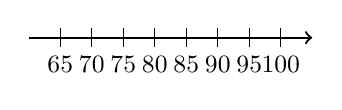
\begin{tikzpicture}[scale=0.08]
  \draw[thick,->] (60,0) -- (105,0);
  \foreach \x in {65,70,...,100} {
    \draw (\x,1.5) -- (\x,-1.5) node[below,font=\small] {$\x$};
  }
\end{tikzpicture}
\end{center}
\end{questionText}
\correctAnswer{$s \geq 87$; closed circle at $87$, shade right}
\explanation{$\frac{78 + 85 + 90 + s}{4} \geq 85$. Multiply by $4$: $253 + s \geq 340$. Subtract $253$: $s \geq 87$. Closed circle at $87$, shade right.}
\end{practiceQuestion}

\begin{practiceQuestion}{6-1-q24}{sa}
\begin{questionText}
A drawing of a room uses scale $1$ cm $= 3$ m. The drawing shows a square room with side $4$ cm. If the scale factor doubles all lengths, by what factor does the actual area change?
\end{questionText}
\correctAnswer{The area does not change}
\explanation{The actual room stays the same. Changing the drawing scale does not change the real room's area. The area of the real room is always $12 \times 12 = 144$ m$^2$.}
\end{practiceQuestion}

\begin{practiceQuestion}{6-2-q05}{mc}
\begin{questionText}
When you redraw a scale drawing at a smaller scale (more real units per cm), the new drawing is:
\end{questionText}
\choiceA{Larger than the original drawing}
\choiceB{Smaller than the original drawing}
\choiceC{The same size as the original drawing}
\choiceD{A different shape than the original drawing}
\correctAnswer{B}
\explanation{A smaller scale means each cm represents more real distance, so fewer cm are needed. The drawing gets smaller. The shape stays the same.}
\end{practiceQuestion}

\begin{practiceQuestion}{6-5-q06}{mc}
\begin{questionText}
You slice a cube with a vertical cut from one face to the opposite face, perpendicular to the base. What is the most likely cross-section shape?
\end{questionText}
\choiceA{Square or rectangle}
\choiceB{Circle}
\choiceC{Triangle}
\choiceD{Hexagon}
\correctAnswer{A}
\explanation{A vertical cut through a cube perpendicular to the base typically produces a rectangle. If the cut goes through the center parallel to a face, it can be a square.}
\end{practiceQuestion}

\begin{practiceQuestion}{6-6-q06}{mc}
\begin{questionText}
Which pair of angles are supplementary?
\end{questionText}
\choiceA{$45°$ and $45°$}
\choiceB{$60°$ and $30°$}
\choiceC{$110°$ and $70°$}
\choiceD{$100°$ and $100°$}
\correctAnswer{C}
\explanation{Supplementary angles sum to $180°$. $110 + 70 = 180$ \checkmark. The others: $45 + 45 = 90$, $60 + 30 = 90$, $100 + 100 = 200$. Only C works.}
\end{practiceQuestion}

\begin{practiceQuestion}{6-7-q10}{mc}
\begin{questionText}
Point $H(-3, 7)$ is reflected over the $y$-axis. What are the coordinates of $H'$?
\end{questionText}
\choiceA{$(-3, -7)$}
\choiceB{$(3, 7)$}
\choiceC{$(3, -7)$}
\choiceD{$(7, -3)$}
\correctAnswer{B}
\explanation{Over the $y$-axis: negate $x$, keep $y$. $(-3, 7) \to (3, 7)$.}
\end{practiceQuestion}

\begin{practiceQuestion}{6-8-q20}{sa}
\begin{questionText}
A tree casts a $16$-ft shadow. A $4$-ft fence post casts a $5$-ft shadow at the same time. How tall is the tree? Round to the nearest tenth.
\end{questionText}
\correctAnswer{$12.8$ ft}
\explanation{$\frac{4}{5} = \frac{h}{16}$. Cross-multiply: $5h = 64$. Divide: $h = 12.8$ ft.}
\end{practiceQuestion}

\begin{practiceQuestion}{7-4-q04}{mc}
\begin{questionText}
A shape is made of a square with side $8$ cm and a semicircle with diameter $8$ cm attached to one side. What is the area? Use $\pi \approx 3.14$.
\end{questionText}
\choiceA{$64$ cm$^2$}
\choiceB{$89.12$ cm$^2$}
\choiceC{$114.24$ cm$^2$}
\choiceD{$139.12$ cm$^2$}
\correctAnswer{B}
\explanation{Square: $8^2 = 64$ cm$^2$. Semicircle: $\frac{1}{2} \times \pi r^2 = \frac{1}{2} \times 3.14 \times 16 = 25.12$ cm$^2$. Total: $64 + 25.12 = 89.12$ cm$^2$.}
\end{practiceQuestion}

\begin{practiceQuestion}{7-5-q17}{mc}
\begin{questionText}
A paint company needs to paint the outside of a box that is $3$ m by $2$ m by $1$ m. Each can of paint covers $5$ m$^2$. How many cans are needed?
\end{questionText}
\choiceA{$3$}
\choiceB{$4$}
\choiceC{$5$}
\choiceD{$6$}
\correctAnswer{C}
\explanation{$SA = 2(3 \times 2) + 2(3 \times 1) + 2(2 \times 1) = 12 + 6 + 4 = 22$ m$^2$. Cans: $22 \div 5 = 4.4$. Round up to $5$ cans.}
\end{practiceQuestion}

\begin{practiceQuestion}{7-6-q24}{sa}
\begin{questionText}
A planter box is $3$ ft long, $1.5$ ft wide, and $2$ ft deep. How many cubic feet of soil are needed to fill it?
\end{questionText}
\correctAnswer{$9$ ft$^3$}
\explanation{$V = 3 \times 1.5 \times 2 = 9$ ft$^3$.}
\end{practiceQuestion}

\begin{practiceQuestion}{7-7-q05}{mc}
\begin{questionText}
Which part of the surface area formula $SA = 2\pi r^2 + 2\pi rh$ represents the area of the two circular bases?
\end{questionText}
\choiceA{$2\pi rh$}
\choiceB{$2\pi r^2$}
\choiceC{$\pi r^2 h$}
\choiceD{$\pi r^2$}
\correctAnswer{B}
\explanation{$2\pi r^2$ gives the area of both circular bases (each base has area $\pi r^2$, and there are $2$ of them).}
\end{practiceQuestion}

\begin{practiceQuestion}{8-1-q25}{sa}
\begin{questionText}
A factory produces $10{,}000$ batteries per day. A sample of $200$ batteries is tested, and $8$ are defective. What percent of the sample is defective?
\end{questionText}
\correctAnswer{$4\%$}
\explanation{$\frac{8}{200} = 0.04 = 4\%$.}
\end{practiceQuestion}

\begin{practiceQuestion}{8-3-q27}{gmc}
\begin{questionText}
The dot plots below show the number of push-ups completed by students in two gym classes.

\begin{center}
\begin{tikzpicture}[scale=0.55]
  % Class 1
  \node[left,font=\small\bfseries] at (4,2.5) {Class 1};
  \draw[thick,->] (4.5,0) -- (16.5,0);
  \foreach \x in {5,6,...,16} {
    \draw (\x,0.1) -- (\x,-0.1);
    \node[below,font=\tiny] at (\x,0) {$\x$};
  }
  % Class 1 data: 7(1),8(2),9(3),10(4),11(3),12(2),13(1)
  \fill[funBlue] (7,0.4) circle (0.15);
  \fill[funBlue] (8,0.4) circle (0.15); \fill[funBlue] (8,0.75) circle (0.15);
  \fill[funBlue] (9,0.4) circle (0.15); \fill[funBlue] (9,0.75) circle (0.15); \fill[funBlue] (9,1.1) circle (0.15);
  \fill[funBlue] (10,0.4) circle (0.15); \fill[funBlue] (10,0.75) circle (0.15); \fill[funBlue] (10,1.1) circle (0.15); \fill[funBlue] (10,1.45) circle (0.15);
  \fill[funBlue] (11,0.4) circle (0.15); \fill[funBlue] (11,0.75) circle (0.15); \fill[funBlue] (11,1.1) circle (0.15);
  \fill[funBlue] (12,0.4) circle (0.15); \fill[funBlue] (12,0.75) circle (0.15);
  \fill[funBlue] (13,0.4) circle (0.15);

  % Class 2
  \node[left,font=\small\bfseries] at (4,5.5) {Class 2};
  \draw[thick,->] (4.5,3.5) -- (16.5,3.5);
  \foreach \x in {5,6,...,16} {
    \draw (\x,3.6) -- (\x,3.4);
    \node[below,font=\tiny] at (\x,3.4) {};
  }
  % Class 2 data: 10(1),11(2),12(3),13(4),14(3),15(2),16(1)
  \fill[funGreen] (10,3.9) circle (0.15);
  \fill[funGreen] (11,3.9) circle (0.15); \fill[funGreen] (11,4.25) circle (0.15);
  \fill[funGreen] (12,3.9) circle (0.15); \fill[funGreen] (12,4.25) circle (0.15); \fill[funGreen] (12,4.6) circle (0.15);
  \fill[funGreen] (13,3.9) circle (0.15); \fill[funGreen] (13,4.25) circle (0.15); \fill[funGreen] (13,4.6) circle (0.15); \fill[funGreen] (13,4.95) circle (0.15);
  \fill[funGreen] (14,3.9) circle (0.15); \fill[funGreen] (14,4.25) circle (0.15); \fill[funGreen] (14,4.6) circle (0.15);
  \fill[funGreen] (15,3.9) circle (0.15); \fill[funGreen] (15,4.25) circle (0.15);
  \fill[funGreen] (16,3.9) circle (0.15);
\end{tikzpicture}
\end{center}

Which class has a higher center, and by approximately how many push-ups?
\end{questionText}
\choiceA{Class 1, by about $3$}
\choiceB{Class 2, by about $3$}
\choiceC{Class 2, by about $6$}
\choiceD{They have the same center}
\correctAnswer{B}
\explanation{Class 1 center $\approx 10$. Class 2 center $\approx 13$. Difference $\approx 3$ push-ups. Class 2 is higher.}
\end{practiceQuestion}

\begin{practiceQuestion}{8-4-q29}{gsa}
\begin{questionText}
The dot plots show daily high temperatures (°F) for two cities over $10$ days.

\begin{center}
\begin{tikzpicture}[scale=0.45]
  % City A
  \node[left,font=\small\bfseries] at (57,2) {City A};
  \draw[thick,->] (57,0) -- (77,0);
  \foreach \x in {58,60,...,76} {
    \draw (\x,0.15) -- (\x,-0.15);
    \node[below,font=\tiny] at (\x,0) {$\x$};
  }
  % City A: 62,64,64,66,66,66,68,68,70,72  mean=66.6
  \fill[funBlue] (62,0.4) circle (0.18);
  \fill[funBlue] (64,0.4) circle (0.18); \fill[funBlue] (64,0.8) circle (0.18);
  \fill[funBlue] (66,0.4) circle (0.18); \fill[funBlue] (66,0.8) circle (0.18); \fill[funBlue] (66,1.2) circle (0.18);
  \fill[funBlue] (68,0.4) circle (0.18); \fill[funBlue] (68,0.8) circle (0.18);
  \fill[funBlue] (70,0.4) circle (0.18);
  \fill[funBlue] (72,0.4) circle (0.18);

  % City B
  \node[left,font=\small\bfseries] at (57,5.5) {City B};
  \draw[thick,->] (57,3.5) -- (77,3.5);
  \foreach \x in {58,60,...,76} {
    \draw (\x,3.65) -- (\x,3.35);
  }
  % City B: 58,60,64,66,68,70,72,74,74,76  mean=68.2
  \fill[funOrange] (58,3.9) circle (0.18);
  \fill[funOrange] (60,3.9) circle (0.18);
  \fill[funOrange] (64,3.9) circle (0.18);
  \fill[funOrange] (66,3.9) circle (0.18);
  \fill[funOrange] (68,3.9) circle (0.18);
  \fill[funOrange] (70,3.9) circle (0.18);
  \fill[funOrange] (72,3.9) circle (0.18);
  \fill[funOrange] (74,3.9) circle (0.18); \fill[funOrange] (74,4.3) circle (0.18);
  \fill[funOrange] (76,3.9) circle (0.18);
\end{tikzpicture}
\end{center}

Find the mean and range for each city. Which city has more consistent temperatures?
\end{questionText}
\correctAnswer{City A: mean $= 66.6$°F, range $= 10$°F. City B: mean $= 68.2$°F, range $= 18$°F. City A is more consistent.}
\explanation{City A: $(62+64+64+66+66+66+68+68+70+72) \div 10 = 666 \div 10 = 66.6$. Range $= 72 - 62 = 10$. City B: $(58+60+64+66+68+70+72+74+74+76) \div 10 = 682 \div 10 = 68.2$. Range $= 76 - 58 = 18$. City A has the smaller range.}
\end{practiceQuestion}

\begin{practiceQuestion}{8-5-q01}{mc}
\begin{questionText}
In a stem-and-leaf plot, $5 \mid 3$ means:
\end{questionText}
\choiceA{$5.3$}
\choiceB{$35$}
\choiceC{$53$}
\choiceD{$5 + 3 = 8$}
\correctAnswer{C}
\explanation{The stem is the tens digit and the leaf is the ones digit, so $5 \mid 3$ means $53$.}
\end{practiceQuestion}

\begin{practiceQuestion}{9-3-q14}{mc}
\begin{questionText}
A die is rolled $120$ times. Each number appears the following number of times: $1$: $22$, $2$: $18$, $3$: $20$, $4$: $21$, $5$: $19$, $6$: $20$. Which number had the highest experimental probability?
\end{questionText}
\choiceA{$1$}
\choiceB{$3$}
\choiceC{$4$}
\choiceD{$6$}
\correctAnswer{A}
\explanation{The number $1$ appeared $22$ times, the most of any number. $P(1) = \frac{22}{120} \approx 0.183$.}
\end{practiceQuestion}

\begin{practiceQuestion}{9-6-q27}{gmc}
\begin{questionText}
The tree diagram shows the outcomes for flipping two coins. What is the probability of getting at least one tail?

\begin{center}
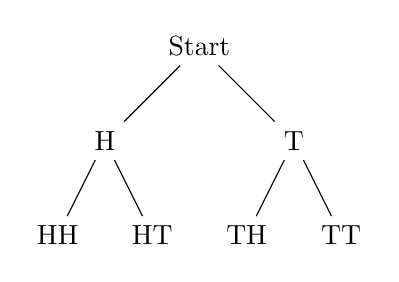
\begin{tikzpicture}[scale=0.8,
  level 1/.style={sibling distance=3cm, level distance=1.5cm},
  level 2/.style={sibling distance=1.5cm, level distance=1.5cm}]
  \node {Start}
    child {node {H}
      child {node {HH}}
      child {node {HT}}
    }
    child {node {T}
      child {node {TH}}
      child {node {TT}}
    };
\end{tikzpicture}
\end{center}
\end{questionText}
\choiceA{$\frac{1}{4}$}
\choiceB{$\frac{1}{2}$}
\choiceC{$\frac{3}{4}$}
\choiceD{$\frac{2}{4}$}
\correctAnswer{C}
\explanation{Outcomes with at least one tail: HT, TH, TT — that is $3$ out of $4$. $P = \frac{3}{4}$.}
\end{practiceQuestion}

\begin{practiceQuestion}{9-7-q27}{gmc}
\begin{questionText}
The bar graph shows the results of simulating a spinner $100$ times. The spinner is supposed to land on each color with equal probability. Based on the simulation, does the spinner appear fair?

\begin{center}
\begin{tikzpicture}[scale=0.55]
  \draw[thick,->] (0,0) -- (0,32) node[above,font=\small] {Frequency};
  \draw[thick,->] (0,0) -- (7,0);
  \foreach \y in {5,10,...,30} {
    \draw[gray!30] (0,\y) -- (6.5,\y);
    \node[left,font=\small] at (0,\y) {\y};
  }
  \fill[funRed!70] (0.5,0) rectangle (1.5,26);
  \fill[funBlue!70] (2.5,0) rectangle (3.5,24);
  \fill[funGreen!70] (4.5,0) rectangle (5.5,28);
  \node[below,font=\small] at (1,0) {Red};
  \node[below,font=\small] at (3,0) {Blue};
  \node[below,font=\small] at (5,0) {Grn.};
  \node[below,font=\small] at (3,-1) {Not shown: Yellow $= 22$};
\end{tikzpicture}
\end{center}
\end{questionText}
\choiceA{No, because the bars are different heights}
\choiceB{Yes, the frequencies ($26, 24, 28, 22$) are all roughly close to $25$}
\choiceC{No, Green is clearly the most likely color}
\choiceD{Cannot be determined from the graph}
\correctAnswer{B}
\explanation{With $4$ equal sections, each should appear about $25$ times in $100$ spins. The results ($26, 24, 28, 22$) are all close to $25$, suggesting the spinner is fair.}
\end{practiceQuestion}
